\documentclass[tikz]{standalone}
\usepackage{pgfplots}
\pgfplotsset{compat=1.15}
\usepackage{mathrsfs}
\usetikzlibrary{arrows,calc}
\usepackage{tkz-euclide}

\pagestyle{empty}

\definecolor{AngleClr}{rgb}{0,0.39215686274509803,0}
\definecolor{ShapeClr}{rgb}{0.6,0.2,0}

\begin{document}

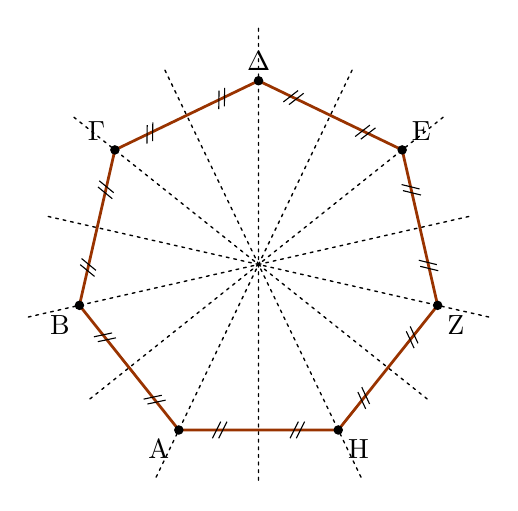
\begin{tikzpicture}[scale=.75]
\tkzSetUpLine[line width=1pt,color=black]
\tkzSetUpPoint[fill=black]

\tkzDefPoints{0/0/P0,2.7/0/P1}
\tkzDefRegPolygon[side,sides=7](P0,P1)

\tkzDefMidPoint(P1,P2) \tkzGetPoint{M1}
\tkzDefMidPoint(P2,P3) \tkzGetPoint{M2}
\tkzDefMidPoint(P3,P4) \tkzGetPoint{M3}
\tkzDefMidPoint(P4,P5) \tkzGetPoint{M4}
\tkzDefMidPoint(P5,P6) \tkzGetPoint{M5}
\tkzDefMidPoint(P6,P7) \tkzGetPoint{M6}
\tkzDefMidPoint(P7,P1) \tkzGetPoint{M7}

\tkzFillPolygon[fill=white](P1,P2,P3,P4,P5,P6,P7)

\tkzDrawSegments[line width=0.5pt,color=black,dashed,dash pattern=on 1pt off 1.75pt,add=0.15 and 0.15](P1,M4 P2,M5 P3,M6 P4,M7 P5,M1 P6,M2 P7,M3)


\tkzDrawPolygon[color=ShapeClr](P1,P2,P3,P4,P5,P6,P7)

\tkzDrawPoints[size=3](P1,P2,P3,P4,P5,P6,P7)
\tkzLabelPoint[below left](P1){$\rm A$}
\tkzLabelPoint[below right](P2){$\rm H$}
\tkzLabelPoint[below right](P3){$\rm Z$}
\tkzLabelPoint[above right](P4){$\rm E$}
\tkzLabelPoint[above](P5){$\rm \Delta$}
\tkzLabelPoint[above left](P6){$\rm \Gamma$}
\tkzLabelPoint[below left](P7){$\rm B$}

\tkzMarkSegments[mark=s||,size=3](P1,M1 P2,M1 P2,M2 P3,M2 P3,M3 P4,M3 P4,M4 M4,P5 P5,M5 M5,P6 P6,M6 M6,P7 P7,M7 M7,P1)

\end{tikzpicture}

\end{document}
